\scanpage{57}
\figure{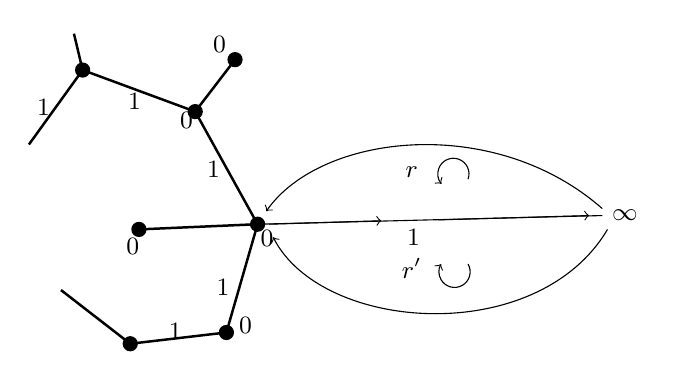
\begin{tikzpicture}[scale=1.1,every node/.style={font=\small}]
\draw[line width=.9pt] (-1.5,3.4)--(-1.4,2.98)--(-.1,2.5)--(.62,1.2)--(.26,-.05)--(-.85,-.18)--(-1.65,.44);
\draw[line width=.9pt] (-1.4,2.98)--(-2.02,2.12) (-.1,2.5)--(.36,3.1) (.62,1.2)--(-.75,1.14);
\draw (.62,1.2)--(4.6,1.3);
\draw[->] (.75,1.2)--(2.05,1.24);\draw[->] (2.7,1.25)--(4.45,1.3);
\draw[->] (4.6,1.38) .. controls (3.35,2.48) and (1.35,2.25) .. (.72,1.35);
\draw[->] (4.66,1.14) .. controls (3.85,-.23) and (1.36,-.05) .. (.8,1.05);
\node at (2.4,1.8) {$r$};\node at (2.4,.69) {$r'$};
\draw[->] (3.05,1.72) arc (-20:220:.18);\draw[->] (3.05,.74) arc (30:-210:.18);
\foreach \x/\y in {-1.4/2.98,-.1/2.5,.36/3.1,.62/1.2,-.75/1.14,.26/-.05,-.85/-.18}{\fill (\x,\y) circle(2.5pt);}
\foreach \x/\y in {-.2/2.4,.18/3.27,.73/1.04,-.82/.94,.48/.03}{\node at (\x,\y) {$0$};}
\foreach \x/\y in {-1.85/2.55,-.8/2.62,.11/1.83,.22/.47,-.33/-.04,2.42/1.05}{\node at (\x,\y) {$1$};}
\node[right] at (4.6,1.3) {$\infty$};
\end{tikzpicture}}
\[
(10)\quad\left\{\begin{aligned}
r'&=\tau_\infty r=\tau_0r\deleted{\unsure{r}}\\
\text{i.e.}\quad\tau_0\tau_\infty r&=r\quad\text{i.e.}\quad\rho_1r=r
\end{aligned}\right.
\]
\deleted{\figure{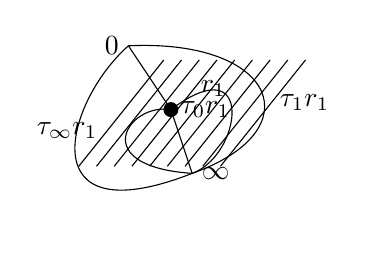
\begin{tikzpicture}[scale=.9]
\draw (0,1.8)--(.6,.9)--(.9,0);
\fill (.6,.9) circle(3pt);
\draw (0,1.8) .. controls (2.1,1.9) and (2.6,.6) .. (.9,0) .. controls (-1.4,-.9) and (-.9,1) .. (0,1.8);
\draw (.6,.9) .. controls (1.8,1.8) and (1.6,.25) .. (.9,0) .. controls (-.6,.1) and (0,1) .. (.6,.9);
\node[left] at (0,1.8) {$0$};\node[right] at (.9,0) {$\infty$};
\node at (1.2,1.2) {$r_1$};\node[left] at (-.3,.6) {$\tau_\infty r_1$};\node[right] at (.6,.9) {$\unsure{\tau_0r_1}$};\node[right] at (2,1) {$\unsure{\tau_1r_1}$};
\foreach \x in {-.7,-.45,...,1.3}{\draw (\x,.1)--(\x+1.2,1.6);}
\end{tikzpicture}}}

Les arêtes \unsure{aplaties} correspondent 1-1 aux ``sommets de type 1'' (de la subdivision barycentrique) qui sont des sommets topologiques (néc\textsuperscript{t}. d'ordre 1) de $K$. Et elles correspondent 1-1 aux points fixes de $\rho_1=\unsure{\sigma_0\sigma_\infty|\tau_0\tau_\infty}$ opérant sur $R$.

Pour un pt. bout de $K$ qui est un sommet marqué de $K$ (i.e. un sommet de type 1 de la subdivision barycentrique) on a la situation ci-contre
\figure{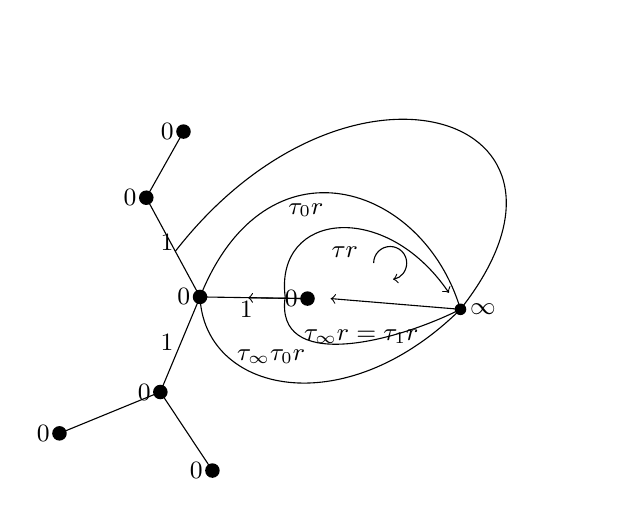
\begin{tikzpicture}[scale=1.05,every node/.style={font=\small}]
\draw (-.2,2.5)--(-.65,1.7)--(0,.5)--(-.48,-.65)--(-1.7,-1.15) (-.48,-.65)--(.15,-1.6) (0,.5)--(1.3,.48);
\foreach \x/\y in {-.2/2.5,-.65/1.7,0/.5,-.48/-.65,-1.7/-1.15,.15/-1.6,1.3/.48}{\fill (\x,\y) circle(2.5pt);\node[left] at (\x,\y) {$0$};}
\foreach \x/\y in {-.4/1.16,-.4/-.05,.56/.35}{\node at (\x,\y) {$1$};}
\draw (-.3,1.05) .. controls (1.8,3.75) and (5,2.7) .. (3.15,.35);
\draw (0,.5) .. controls (.8,2.5) and (2.7,1.87) .. (3.15,.35) .. controls (1.73,-1.05) and (.05,-.65) .. (0,.5);
\draw[->] (3.15,.35)--(1.58,.48);
\draw[->] (1.26,.48)--(.58,.49);
\draw[->] (1.03,.5) .. controls (.9,1.53) and (2.24,1.68) .. (3.01,.55);
\draw (1.03,.5) .. controls (.9,-.4) and (2.31,-.07) .. (3.15,.35);
\fill (3.15,.35) circle(2pt);\node[right] at (3.15,.35) {$\infty$};
\node at (1.28,1.55) {$\tau_0r$};\node at (1.75,1.04) {$\deleted{\unsure{\tau}}r$};
\draw[->] (2.1,.91) arc (180:-80:.2);
\node at (.86,-.22) {$\tau_\infty\tau_0r$};\node at (1.95,.02) {$\unsure{\tau_\infty r=\tau_1r}$};
\end{tikzpicture}}
, il y a bien \uline{4} repères distincts adjacents à l'arête qui aboutit en ce sommet -- si on prend l'un des deux qui \deleted{\unsure{ont pour}} \inserted{ont comme} \deleted{``plié''} \inserted{``pli''} le \deleted{sommet} envisagé, on aura
\[
(11)\qquad\tau_1r=\tau_\infty r\qquad\text{i.e.}\quad\rho_0r=r
\]
ce qui caractérise les sommets envisagés (ils sont en corr. biunivoque avec les paires de repères $\{r,r'\}$ telles que $r'=\tau_1r=\tau_\infty r$, d'où $r=\tau_1r'=\tau_\infty r'$).

\deleted{\unsure{La condition}} La condition (11) n'\unsure{empêche} pas qu'on

\mspage{56}
